%% 《高级图论》课程论文 V2
%% 基于《计算机学报》单栏 CjC 模板（Overleaf: latextemplet-CjC-xelatex）
%% 编译方式：XeLaTeX；请将本文件与 figures/、ref.bib 放入模板工程后编译
\documentclass[10.5pt,compsoc,UTF8]{CjC}
\usepackage{CTEX}
\usepackage{graphicx}
\usepackage{footmisc}
\usepackage{subfigure}
\usepackage{url}
\usepackage{multirow}
\usepackage{multicol}
\usepackage[noadjust]{cite}
\usepackage{amsmath,amsthm}
\usepackage{amssymb,amsfonts}
\usepackage{booktabs}
\usepackage{color}
\usepackage{ccaption}
\usepackage{float}
\usepackage{fancyhdr}
\usepackage{caption}
\usepackage{xcolor,stfloats}
\usepackage{comment}
\setcounter{page}{1}
\graphicspath{{figures/}}
\usepackage{cuted}
\usepackage{captionhack}
\usepackage{epstopdf}
\usepackage{gbt7714}

%===============================%
\headevenname{\mbox{\quad} \hfill  \mbox{\zihao{-5}{ \hfill 《高级图论》课程论文  } \hspace {50mm} \mbox{2026 年 7 月}}}%
\headoddname{杜浩存 \hfill 基于图结构的任意字段集合敏感度评估与高阶协同泄露推断}%

\renewcommand{\thefootnote}{\fnsymbol{footnote}}
\setcounter{footnote}{0}
\renewcommand\footnotelayout{\zihao{5-}}

\newtheoremstyle{mystyle}{6pt}{6pt}{\normalfont}{1em}{\bf}{}{1em}{}
\theoremstyle{mystyle}
\newtheorem{definition}{定义}
\newtheorem{observation}{观察}
\renewcommand\figurename{图~}
\renewcommand{\thesubfigure}{(\alph{subfigure})}
\newcommand{\upcite}[1]{\textsuperscript{\cite{#1}}}
\renewcommand{\labelenumi}{(\arabic{enumi})}
\newcommand{\tabincell}[2]{\begin{tabular}{@{}#1@{}}#2\end{tabular}}
\renewcommand{\bibsection}{}
\makeatletter
\renewcommand{\@biblabel}[1]{[#1]\hfill}
\makeatother
\setlength\parindent{2em}

\begin{document}

\hyphenpenalty=50000
\thispagestyle{plain}%
\thispagestyle{empty}%
\pagestyle{CjCheadings}

\vspace {-13mm}
\onecolumn
\zihao{5-}\noindent 杜浩存 \hfill 《高级图论》课程论文\hfill 2026 年 7 月\\
\noindent\rule[0.25\baselineskip]{\textwidth}{1pt}

{
\centering
\vspace {11mm}
{\zihao{2} \heiti 基于图结构的电网数据任意字段集合敏感度评估\\与高阶协同泄露推断}

\vskip 5mm

{\zihao{4}\fangsong 杜浩存}

\vspace {5mm}

\zihao{5}{(西安交通大学\quad 西安\quad 710049)}
}

\vskip 5mm

\zihao{5}{
\setlength{\baselineskip}{16pt}\selectfont{
\noindent {\heiti 摘\quad 要\quad }
电网运行数据在共享前通常仅删除机密字段，然而剩余字段之间由物理定律与统计规律决定的耦合关系，使攻击者仍能训练推断模型间接恢复机密量，即数据推断泄露。现有敏感度评估方法（如 IGNN）为每个字段输出一个标量敏感度分数，本文通过对 PJM 电网 44 字段真实数据的系统测量指出这一刻画方式的不适定性：泄露风险本质上是可见字段\textbf{集合}上的集合函数，存在强烈的“单看安全、合体泄露”协同效应——风电出力与风电占比两字段单独推断总发电量的测试 $R^2$ 仅为 0.064 与 0.162，合并后升至 0.928。为忠实刻画并高效评估这一集合函数，本文提出一个以图结构为骨架的三阶段评估框架。阶段一融合五种相关性度量构建字段相关图，为后续模型提供结构先验；阶段二在该图上建立集合敏感度的双通道评估机制：以逐集合重训的可见性感知图推断模型作为敏感度真值（攻击者最优响应语义），以随机子集失活联合训练的子集条件图 oracle 配合 $K$ 步查询微调作为秒级估计器，将单集合评估成本较完整重训压缩两个数量级以上（$K{=}200$ 时每集合约 3 秒，逐机密字段平均绝对误差 0.078，集合排序 Spearman 相关系数达 0.97 以上）；阶段三提出“估计器全扫描 + 重训认证”协议，在 $\binom{44}{3}=13244$ 个三元组的组合空间中定位真不可约三阶协同并给出重训证书。实验表明：估计与认证排序的 Spearman 相关系数为 0.795 且估计系统性保守，认证发现的最强三阶协同“燃气出力 + 燃气占比 + 负荷预测 $\to$ 净交换功率”达 0.455，其物理机制为三字段缺一不可；随机对照组 2400 条认证记录中仅 19 条超过显著阈值，证明高阶协同泄露是稀疏且物理可解释的结构。实验还定量否定了基于置零的评估口径：其协同估计相对重训真值系统性低估 3.4 倍、排序相关系数仅 0.351，表明忠实的集合敏感度评估必须以重训为真值。此外，图结构推断模型在 5 字段以上的集合上较多层感知机基线具有一致的精度优势，且其参数与字段身份解耦，为跨系统迁移提供了结构基础。
\par}}
\vspace {5mm}

\zihao{5}{\noindent
{\heiti 关键词 \quad }图神经网络；数据推断泄露；集合函数；协同效应；数据脱敏；电力信息物理系统
}

\vskip 7mm

\begin{center}
\zihao{3}{ \heiti Graph-Structured Sensitivity Assessment of Arbitrary Field Subsets and Higher-Order Synergistic Leakage Inference for Power Grid Data}\\
\vspace {5mm}
\zihao{5}{ DU Hao-Cun}\\
\vspace {2mm}
\zihao{5-}{{(Xi'an Jiaotong University, Xi'an 710049, China)}}
\end{center}

\zihao{5}{
\setlength{\baselineskip}{18pt}\selectfont{
{\bf Abstract}\quad
Operational power grid data are usually desensitized by simply removing confidential fields before sharing. However, the couplings among the remaining fields, determined by physical laws and statistical regularities, still allow an attacker to train inference models and indirectly recover confidential quantities, a threat known as data inference leakage (DIL). Existing sensitivity assessment methods such as IGNN assign a scalar sensitivity score to each individual field. Through systematic measurements on real PJM data with 44 fields, this paper shows that such a pointwise characterization is ill-posed: leakage risk is essentially a set function over subsets of visible fields, exhibiting strong ``individually harmless, jointly revealing'' synergy --- wind generation (MW) and wind share individually infer total generation with test $R^2$ of only 0.064 and 0.162, yet jointly reach 0.928. To faithfully characterize and efficiently evaluate this set function, this paper proposes a three-stage graph-structured assessment framework. Stage I fuses five correlation measures to construct a field correlation graph as the structural prior. Stage II establishes a dual-channel evaluation mechanism on this graph: a visibility-aware graph inference model retrained per subset serves as the ground truth of sensitivity under the attacker's best-response semantics, while a subset-conditional graph oracle trained with random subset dropout, combined with $K$-step query-time fine-tuning, serves as a second-level estimator that reduces the per-subset evaluation cost by more than two orders of magnitude compared with full retraining (about 3 seconds per subset at $K{=}200$, per-confidential-field MAE 0.078, and subset-ranking Spearman correlation above 0.97). Stage III proposes a ``scan-then-certify'' protocol that locates irreducible third-order synergies in the combinatorial space of $\binom{44}{3}=13244$ triples and issues retraining certificates. Experiments show that the estimated and certified rankings correlate at Spearman 0.795 with the estimator being systematically conservative; the strongest certified third-order synergy, ``gas MW + gas share + load forecast $\to$ net interchange'', reaches 0.455, whose physical mechanism requires all three fields; only 19 of 2400 certified records in the random control group exceed the significance threshold, demonstrating that higher-order synergistic leakage is a sparse and physically interpretable structure. The experiments also quantitatively refute the zeroing-based assessment: it underestimates synergy by 3.4 times with a rank correlation of merely 0.351 against retraining truth, indicating that faithful subset sensitivity assessment must be grounded in retraining. In addition, the graph-structured inference model consistently outperforms an MLP baseline on subsets with five or more fields, and its parameters are decoupled from field identities, providing a structural basis for cross-system transfer.
\par}}
\vspace {5mm}

{{\bf Keywords}\quad graph neural network; data inference leakage; set function; synergy; data desensitization; cyber-physical power system\par}

\zihao{5}
\vskip 10mm

%%%%%%%%%%%%%%%%%%%%%%%%%%%%%%%%%%%%%%%%%%
\section{\heiti 引言}

现代电力系统已经演化为深度互联的信息物理系统（Cyber-Physical Power Grid, CPPG），其发电调度、电力市场与规划运行高度依赖细粒度运行数据在多主体之间的持续交换与共享。共享前的脱敏处理在工程实践中通常被简化为一件事：删除被规程认定为机密的字段。然而，保留下来的“一般字段”之间存在由物理定律（潮流方程、功率平衡、燃料—出力关系）与统计规律（负荷周期性、气象相关性、市场联动）共同决定的强耦合，攻击者完全可以利用公开字段训练推断模型，间接恢复被删除的机密量。这一威胁被称为数据推断泄露（Data Inference Leakage, DIL）\upcite{hu2026ignn}。文献[1]梳理了多起真实事件：Strava 运动热力图这类看似无害的聚合数据曾暴露军事基地的位置与布局；2015 年乌克兰电网攻击的长期侦察阶段，攻击者正是借助低敏感度的系统日志与凭据信息逐步推断出 SCADA 拓扑与操作逻辑。这些事件共同说明：不评估推断泄露就共享“低敏感”数据，可能暴露系统中最关键的信息。

针对 DIL 威胁的敏感度评估，代表性工作是 Hu 等人提出的 IGNN\upcite{hu2026ignn}：构建融合模型驱动与数据驱动相关性的推断关系图，以层次分析法标定初始敏感度，再用图注意力网络将风险沿图传播，最终为\textbf{每个字段}输出一个标量敏感度分数。这一框架首次将字段间推断关系组织为图结构，是本文工作的直接出发点。然而，本文在真实电网数据上的系统测量揭示了“单字段分数”这一输出粒度的根本缺陷：\textbf{泄露不是字段的属性，而是字段集合的属性}。典型实例是：风电出力（MW）与风电占比两个字段，各自单独推断机密字段“总发电量”的测试 $R^2$ 分别仅为 0.064 与 0.162，按任何单字段评分体系都属于低风险；但两者同时可见时 $R^2$ 跃升至 0.928——因为总发电量在物理上恰等于出力除以占比。更极端地，太阳能出力字段单独推断的 $R^2$ 仅 0.006（几乎无泄露），却参与了增量达 0.596 的协同泄露。单字段分数在原理上无法表达此类“单看安全、合体泄露”的结构：无论给这两个字段各自打多低的分，都无法预警它们合体后的风险；反之若为防范合体风险而给每个字段打高分，又会将大量真正无害的共享场景误判为高危。敏感度评估必须升维为\textbf{任意字段集合}上的集合函数。

升维之后，三个相互纠缠的挑战随之而来。\textbf{挑战一（语义忠实性）}：“集合 $S$ 的敏感度”应当刻画攻击者拿到 $S$ 后所能达到的推断能力\textbf{上限}，即允许攻击者针对 $S$ 重新训练至最优的“最优响应”语义；而以固定模型加特征置零来近似这一语义（IGNN 及多数特征归因方法的做法）会产生分布外伪影，本文实验将证明该口径系统性低估协同 3.4 倍、排序相关系数仅 0.351。\textbf{挑战二（组合爆炸）}：$n=44$ 个字段的可见集合有 $2^{44}\approx 1.8\times10^{13}$ 个，而忠实语义要求逐集合重训，单次重训即需分钟级开销，穷举在计算上不可行。\textbf{挑战三（高阶结构定位）}：协同可能存在于二阶以上——本文将实证三字段“缺一不可”的真不可约三阶协同——但 $k$ 阶候选空间以 $\binom{n}{k}$ 增长，且高阶协同的观测值必须刨除全部低阶效应并经受噪声检验，如何在指数空间中\textbf{可靠地}定位并\textbf{认证}少数真协同，是集合语义能否落地的关键。

针对上述挑战，本文提出一个以图结构为骨架的三阶段评估框架（图 1）。其核心设计原则是\textbf{真值层与估计层分离}：估计器只承担筛选职能，一切进入结论的数值都以重训证书落地。具体而言，阶段一融合五种相关性度量构建字段相关图，作为全部后续模型的结构先验（4.2 节）；阶段二建立集合敏感度的双通道评估——通道 A 是逐集合重训的可见性感知图推断模型，给出忠实语义下的敏感度真值（4.3 节），通道 B 是以随机子集失活方式联合训练的子集条件图 oracle，配合 $K$ 步查询时微调，一次前向即可给出任意集合的秒级估计（4.4、4.5 节）；阶段三是“估计器全扫描 + 重训认证”协议，以通道 B 扫描指数空间、以通道 A 认证 top 候选与随机对照，并通过排序一致性与保守性两项可检验条件保证协议可靠（4.6 节）。

本文的主要贡献总结如下：

(1) \textbf{问题形式化}。将电网数据敏感度从单字段分数升维为任意可见集合的集合函数 $v_c(S)$，赋予其攻击者最优响应语义，并在其上定义 $k$ 阶不可约协同、协同图与协同超图，将泄露结构组织为字段集上的图论对象（第 3 节）。

(2) \textbf{忠实测量方法学}。以逐集合重训为真值口径，实测复现噪声底（$\sigma\approx0.002$--$0.004$）并据此设定显著性标尺；对置零口径给出定量否定（低估 3.4 倍、排序相关 0.351），确立“廉价口径只能筛选、结论必须重训认证”的测量纪律（3.4、5.2 节）。

(3) \textbf{子集条件图 oracle 与查询时微调}。单一模型摊销学习“集合 $\mapsto$ 重训敏感度”映射，$K{=}200$ 步微调（每集合约 3 秒）后逐机密字段 MAE 达 0.078、集合排序 Spearman 相关 0.97--0.99，将单集合评估成本较重训压缩两个数量级以上（4.4、4.5、5.3 节）。

(4) \textbf{扫描—认证协议与三阶协同发现}。全扫描 13244 个三元组并重训认证约 400 个，验证协议的排序一致性（Spearman 0.795）与保守性（估计不高于真值，筛选不漏强项）；发现最强真不可约三阶协同“燃气出力 + 燃气占比 + 负荷预测 $\to$ 净交换功率”（0.455），并证明高阶协同是稀疏结构（随机对照组阳性率 19/2400），为先验式剪枝提供依据（4.6、5.4 节）。

本文其余部分组织如下：第 2 节评述相关工作；第 3 节给出威胁模型、问题形式化与预备知识；第 4 节详细阐述三阶段评估框架；第 5 节围绕四个研究问题展开实验评估；第 6 节讨论方法边界与未来方向；第 7 节总结全文。

\section{\heiti 相关工作}

\subsection{CPPG 数据敏感度评估与推断泄露}

CPPG 安全风险评估早期聚焦于外部网络攻击（虚假数据注入、拒绝服务）与系统级脆弱性建模，对数据层面的间接泄露关注有限\upcite{hu2026ignn}。模型驱动的推断研究证明了 DIL 的现实性：Kekatos 等人利用非敏感电价基于经济调度模型反推电网拓扑，后续工作进一步利用公开量测推断电压相量、拓扑、应急容量与发电机参数等关键量（见文献[1]的综述）。IGNN\upcite{hu2026ignn} 将这些分散的推断关系统一组织为推断关系图：节点为数据字段，边为模型驱动（物理方程可推导）与数据驱动（Pearson/Spearman/余弦相似度超过阈值）的推断路径，再以图注意力网络把用层次分析法标定的内在敏感度沿图传播，输出各字段的最终敏感度分数。本文与 IGNN 在“以图组织字段间推断关系”上一脉相承，但存在两点本质差异：其一，输出粒度从单字段分数升维为任意集合的集合函数，从而能够表达协同泄露；其二，测量口径从“固定模型 + 风险传播”改为“逐集合重训的攻击者最优响应”，本文第 5.2 节将定量证明前者会系统性扭曲协同结论。

\subsection{特征子集贡献与交互指标}

可解释机器学习领域长期研究特征子集对模型输出的贡献。SHAP\upcite{lundberg2017shap} 以 Shapley 值为公理化基础将预测归因到单特征；Grabisch 等人\upcite{grabisch1999interaction} 将其推广为任意阶的交互指标；FastSHAP\upcite{jethani2022fastshap} 与 ViT-Shapley\upcite{covert2023vitshapley} 训练摊销网络以单次前向估计 Shapley 值，其“一个模型回答所有子集查询”的思想与本文 oracle 相通。但这一族方法刻画的是\textbf{某个固定模型}在特征扰动下的行为，服务于模型解释；本文的 $v_c(S)$ 允许攻击者对每个 $S$ \textbf{重新训练至最优}，刻画的是数据本身的可推断性上限，服务于安全评估。两种语义在协同问题上的差距正是本文置零对比实验所测量的对象。Datamodels\upcite{ilyas2022datamodels} 在训练数据维度拟合“训练子集 $\mapsto$ 模型性能”的函数，与本文在特征维度拟合“可见子集 $\mapsto$ 攻击精度”构成平行工作，其结论（低阶线性代理意外有效）也与本文观察到的协同稀疏性相呼应。

\subsection{任意条件建模与缺失特征学习}

VAEAC\upcite{ivanov2019vaeac} 与 ACFlow\upcite{li2020acflow} 学习对任意观测子集条件化的生成模型 $p(x_{\bar S}\,|\,x_S)$，GRAPE\upcite{you2020grape} 将缺失特征补全建模为“样本—字段”二部图上的表示学习。本文的子集条件 oracle 在“任意子集条件化”的训练机制上借鉴了这一族方法（随机掩码 + 联合训练），但学习目标不同：不是数据分布本身，而是“集合 $\mapsto$ 重训攻击精度”这一集合函数的摊销近似，且其估计值最终要与重训真值对齐并接受认证检验。

\subsection{图神经网络及其归纳偏置}

GCN\upcite{kipf2017gcn} 与 GAT\upcite{velickovic2018gat} 提供了本文图结构模型的基础算子。Battaglia 等人\upcite{battaglia2018relational} 系统论述了关系归纳偏置的适用条件：当任务的依赖结构与图拓扑对齐时，消息传递以参数共享换取样本效率与组合泛化。Grinsztajn 等人\upcite{grinsztajn2022tabular} 则从表格数据的实证出发提醒：结构先验并非在所有回归任务上都优于无结构基线。这两点共同构成本文对图结构收益进行\textbf{按角色定位}（专用推断模型收益明确、摊销估计器收益有限）的理论背景，详见 5.5 与 6.1 节。

表 1 从评估对象、模型语义与输出粒度三个维度对比了上述方法族与本文工作。

\begin{table}[htbp]
\centering {\heiti 表 1\quad 本文方法与相关方法族的对比}
\vspace {1mm}
\begin{center}
\zihao{5-}
\begin{tabular}{lllll}
\toprule
方法类别 & 代表工作 & 模型语义 & 输出粒度 & 协同泄露刻画 \\
\midrule
字段级敏感度评估 & IGNN\upcite{hu2026ignn} & 固定模型 + 图传播 & 单字段分数 & 不可表达 \\
特征归因与交互 & SHAP\upcite{lundberg2017shap}, FastSHAP\upcite{jethani2022fastshap} & 固定模型 + 特征扰动 & 单特征值/交互指标 & 固定模型语义下扭曲 \\
任意条件建模 & VAEAC\upcite{ivanov2019vaeac}, GRAPE\upcite{you2020grape} & 生成模型 & 条件分布 & 非安全语义 \\
训练子集函数 & Datamodels\upcite{ilyas2022datamodels} & 逐子集重训（训练维度） & 子集$\mapsto$性能 & —— \\
\textbf{本文} & —— & \textbf{逐集合重训最优响应} & \textbf{任意集合 $v_c(S)$} & \textbf{二/三阶重训认证} \\
\bottomrule
\end{tabular}
\label{tab:related}
\end{center}
\end{table}

\section{\heiti 威胁模型、问题形式化与预备知识}

\subsection{威胁模型}

设数据持有方拥有数据表 $X\in\mathbb{R}^{N\times n}$，其 $n$ 个字段构成集合 $F=\{f_1,\dots,f_n\}$（本文 $n=44$），其中由规程认定的机密字段集为 $C\subset F$（本文 $|C|=12$，含总发电量、计量负荷、净交换功率、系统损耗、日前/实时阻塞价格及三类备用总量等），其余为一般字段集 $G=F\setminus C$。数据共享时机密字段被删除，攻击者获得某可见字段集合 $S\subseteq G$ 的完整列数据。

对攻击者作如下能力假设：(1) 拥有与共享数据同分布的历史对齐样本（例如公开的历史市场数据），可用于训练推断模型；(2) 知晓字段的物理语义；(3) 可从任意模型族 $\mathcal{G}$ 中选择并训练模型，即不受限于任何固定的预训练模型。这是对攻击者有利的保守假设：评估在此假设下得到的是泄露风险的上界刻画。防御方的目标是：对任意拟共享集合 $S$，在可接受的计算成本内评估每个机密字段 $c\in C$ 被推断的风险，并定位哪些字段组合构成协同泄露源。

\subsection{集合敏感度及其语义}

\begin{definition}[集合敏感度]
给定机密字段 $c\in C$ 与可见集合 $S\subseteq G$，集合敏感度定义为
\begin{equation}
v_c(S)\;=\;\max\Bigl(0,\ \sup_{g\in\mathcal{G}}\ R^2_{\mathrm{test}}\bigl(g(X_S)\,;\,x_c\bigr)\Bigr),
\label{eq:vcs}
\end{equation}
其中 $X_S$ 为仅保留 $S$ 中字段的数据，$R^2_{\mathrm{test}}$ 为在保留测试集上的决定系数。
\end{definition}

式 (\ref{eq:vcs}) 的上确界取在模型族与训练过程之上，即\textbf{攻击者最优响应}语义：对每个 $S$，攻击者可从头重训至该集合下的最优。实践中以“在多种结构（多层感知机与图结构模型）上分别重训并逐机密字段取较优者”作为 $\sup$ 的经验近似（best-of-struct 口径）。$v_c(\cdot)$ 是布尔格 $(2^{G},\subseteq)$ 上的集合函数；在最优响应语义下它在理论上单调不减（信息不会因增加而变少），实测中因优化噪声呈近似单调。对该格的 $2^{44}$ 个元素逐点重训不可行，这正是第 4 节估计器与协议的动机。

\subsection{协同泄露与协同结构}

\begin{definition}[二阶协同]
字段对 $(i,j)$ 对机密字段 $c$ 的协同增量为
\begin{equation}
\mathrm{syn}_2^c(i,j)\;=\;v_c(\{i,j\})-\max\bigl(v_c(\{i\}),\,v_c(\{j\})\bigr).
\label{eq:syn2}
\end{equation}
\end{definition}

\begin{definition}[$k$ 阶不可约协同]
集合 $T$（$|T|=k\ge 3$）的 $k$ 阶不可约协同为其相对最优 $(k{-}1)$ 阶子集的增量
\begin{equation}
\mathrm{syn}_k^c(T)\;=\;v_c(T)-\max_{T'\subset T,\,|T'|=k-1} v_c(T').
\label{eq:synk}
\end{equation}
特别地，三阶不可约协同 $\mathrm{syn}_3^c(i,j,k)=v_c(\{i,j,k\})-\max\bigl(v_c(\{i,j\}),v_c(\{i,k\}),v_c(\{j,k\})\bigr)$。
\end{definition}

定义 3 采用“减去最优低阶子集”而非 M\"obius 反演式的全交互展开\upcite{grabisch1999interaction}，原因在于安全语义：防御者关心的是“同时放行 $T$ 是否比放行其任何真子集更危险”，$\mathrm{syn}_k>0$ 直接回答该问题，且逐层定义天然支持递归的搜索剪枝（4.6 节）。

\begin{definition}[协同图与协同超图]
以字段为顶点、$w(i,j)=\max_{c\in C}\mathrm{syn}_2^c(i,j)$ 为边权的加权图 $G_{\mathrm{syn}}=(F,E_2)$ 称为协同图；显著三阶协同（$\mathrm{syn}_3$ 超过显著阈值）构成的三元组集合 $E_3$ 与 $F$ 构成 3 一致超图 $H_{\mathrm{syn}}=(F,E_3)$，称为协同超图。
\end{definition}

协同图与协同超图把泄露的组合结构组织为可分析的图论对象：防御问题（如“删除最少字段使全部显著协同失效”）转化为其上的顶点覆盖类问题，而第 5.4 节实证的超边稀疏性则是此类问题可解性的经验基础。

\subsection{测量口径、噪声底与显著性}

集合敏感度的数值高度依赖测量口径。本文对比两种口径。\textbf{重训口径}（本文真值）：对每个待测集合 $S$ 按统一协议从头训练攻击者，实测 $R^2$。\textbf{置零口径}（IGNN 及固定模型归因方法的通行做法）：保持在全字段上训练的模型 $g^{*}_{F}$ 参数不变，将 $S$ 以外的输入置零后测残余精度
\begin{equation}
\tilde v_c(S)\;=\;\max\Bigl(0,\ R^2_{\mathrm{test}}\bigl(g^{*}_{F}(X\odot m_S)\,;\,x_c\bigr)\Bigr),
\label{eq:zero}
\end{equation}
其中 $m_S\in\{0,1\}^{n}$ 为 $S$ 的指示掩码，$\odot$ 为逐列乘。置零口径有两个原理性缺陷：置零输入偏离训练分布（分布外伪影），且固定参数无法表达攻击者针对 $S$ 的重新优化（无最优响应）。第 5.2 节将给出其定量后果。

重训口径自身存在复现噪声：对同一集合以不同随机种子重复重训，实测噪声底为 $\sigma\approx0.002$--$0.004$（$R^2$ 单位）。据此本文设定判读标尺：单点差异超过 0.01（多层感知机）/0.02（图模型，其训练方差略大）方视为显著；协同显著阈值取 $\mathrm{syn}>0.10$，约为噪声底的 25 倍以上，保证结论远离噪声。

\subsection{预备知识：图注意力聚合}

设图 $G=(V,E)$ 上节点 $i$ 的特征为 $\mathbf{h}_i$。图注意力网络\upcite{velickovic2018gat}对邻居 $j\in\mathcal{N}(i)$ 计算注意力系数并加权聚合：
\begin{equation}
\alpha_{ij}=\frac{\exp\bigl(\mathrm{score}(\mathbf{h}_i,\mathbf{h}_j)\bigr)}{\sum_{k\in\mathcal{N}(i)}\exp\bigl(\mathrm{score}(\mathbf{h}_i,\mathbf{h}_k)\bigr)},\qquad
\mathbf{h}'_i=\sigma\Bigl(\sum_{j\in\mathcal{N}(i)}\alpha_{ij}\mathbf{W}\mathbf{h}_j\Bigr),
\label{eq:gat}
\end{equation}
其中 $\mathbf{W}$ 为共享线性变换，$\sigma$ 为非线性激活。本文模型在式 (\ref{eq:gat}) 基础上引入可见性掩码对注意力的重归一化（4.3 节），使聚合系数自适应于字段的可见模式。

\section{\heiti 基于图结构的集合敏感度评估框架}

\subsection{框架总览}

图 1 给出框架总览。阶段一构建字段相关图 $G=(F,E)$，为全部后续模型提供统一的结构先验。阶段二在 $G$ 上建立集合敏感度的双通道评估：通道 A（专用图攻击者）对给定集合从头重训，产出定义 1 语义下的真值，其成本高（分钟级）但地位是唯一的“证书”来源；通道 B（子集条件图 oracle）以单一模型摊销全部集合的估计，成本低（秒级）但存在系统性残差，地位是筛选器。阶段三的扫描—认证协议将两个通道组织为闭环：通道 B 全扫描组合空间并排序，通道 A 对 top 候选与随机对照重训认证，认证结果同时检验协议自身的可靠性（排序一致性与保守性）。这一“估计只用于筛选、结论以重训证书落地”的分层设计，是本框架在忠实性与可扩展性之间的核心权衡。

\begin{figure}[htbp]
\centering
\centerline{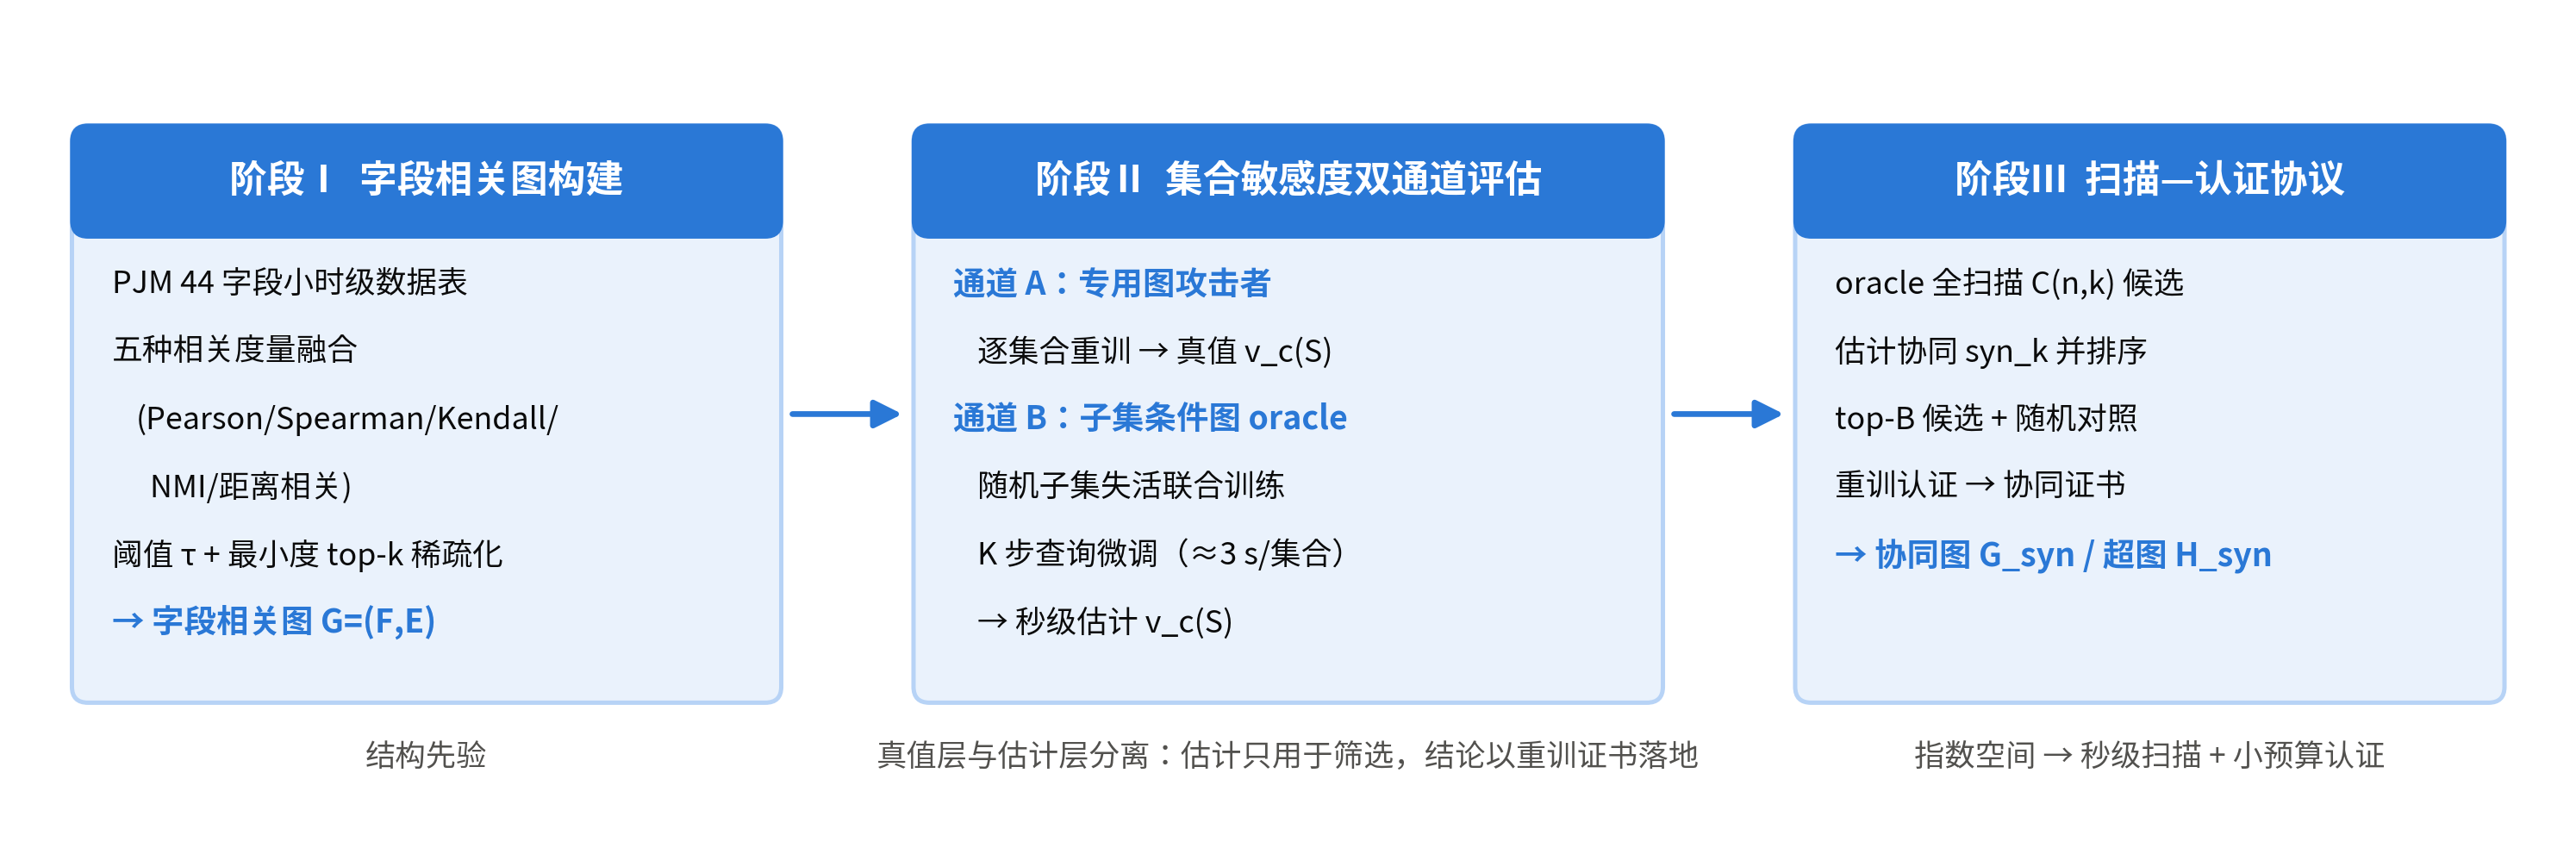
\includegraphics[width=0.98\linewidth]{framework_zh.png}}
{\heiti 图 1\quad 基于图结构的集合敏感度评估框架总览：阶段Ⅰ构建字段相关图；阶段Ⅱ以“重训真值通道 + oracle 估计通道”双通道评估任意集合敏感度；阶段Ⅲ以扫描—认证协议在组合空间中定位并认证高阶协同}
\label{fig:framework}
\end{figure}

\subsection{阶段一：字段相关图构建}

字段间的推断关系既包含线性相关，也包含比值、饱和等非线性耦合，单一相关系数不足以刻画。对每对字段 $(i,j)$ 计算五种相关性度量——Pearson、Spearman、Kendall 相关系数、归一化互信息（NMI）与距离相关（distance correlation）——并取平均：
\begin{equation}
A_{\mathrm{raw}}(i,j)\;=\;\frac{1}{|\mathcal{M}|}\sum_{\mu\in\mathcal{M}}\bigl|\rho_{\mu}(x_i,x_j)\bigr|,
\label{eq:corr}
\end{equation}
其中 $\mathcal{M}$ 为上述度量集合。前三者捕获单调关联，NMI 与距离相关捕获一般非线性依赖，融合后对“占比—出力—总量”这类比值型物理关系仍保持敏感。

在 $A_{\mathrm{raw}}$ 上以“阈值或 top-$k$”规则稀疏化得到边集：
\begin{equation}
E\;=\;\bigl\{(i,j)\,:\,A_{\mathrm{raw}}(i,j)\ge\tau\bigr\}\ \cup\ \bigl\{(i,j)\,:\,j\in\mathrm{top}\text{-}k_{\min}(i)\bigr\},
\label{eq:edge}
\end{equation}
本文取 $\tau=0.15$、$k_{\min}=8$ 并对称化。阈值项保证强关联均入图，top-$k$ 项保证每个顶点的最小度——若无此项，与其余字段相关性普遍偏弱的字段将成为孤立点，其参与的推断路径被先验切断。需要强调 $G$ 的角色定位：它是消息传递的\textbf{结构先验}而非因果图；协同泄露恰恰可能发生在两两相关都弱的字段之间（如太阳能出力对），因此框架不依赖 $G$ 的边权做任何敏感度结论，结论一律由阶段二、三的重训产生。

\subsection{阶段二（通道 A）：可见性感知图推断模型}

通道 A 的模型以 $G$ 为骨架，对给定可见集合 $S$ 从头训练，扮演定义 1 中的攻击者。

\textbf{输入编码}。每个字段为一个节点。给定掩码 $m=m_S$，节点 $i$ 的初始表示编码“观测值 + 可见位”二元组：
\begin{equation}
\mathbf{h}_i^{(0)}\;=\;\phi\bigl([\,x_i\cdot m_i;\ m_i\,]\bigr),
\label{eq:enc}
\end{equation}
其中 $\phi$ 为共享的两层编码器。显式输入 $m_i$ 使模型能够区分“取值为零”与“不可见”，这是掩码条件化的关键。

\textbf{可见性感知注意力}。在层 $l$，节点 $i$ 只从\textbf{可见}邻居聚合信息，注意力在可见邻居上重归一化：
\begin{equation}
\alpha_{ij}^{(l)}(m)\;=\;\frac{m_j\exp\bigl(\mathrm{score}^{(l)}(\mathbf{h}_i^{(l)},\mathbf{h}_j^{(l)})/T\bigr)}{\sum_{k\in\mathcal{N}(i)}m_k\exp\bigl(\mathrm{score}^{(l)}(\mathbf{h}_i^{(l)},\mathbf{h}_k^{(l)})/T\bigr)},
\label{eq:visatt}
\end{equation}
其中 $T$ 为温度超参数。与式 (\ref{eq:gat}) 相比，掩码 $m_j$ 把不可见邻居从 softmax 的分母中移除，使同一组注意力参数在不同掩码模式下自动重新分配聚合权重——这是“一张图适配任意可见模式”的机制基础。层间传播为
\begin{equation}
\mathbf{h}_i^{(l+1)}\;=\;\sigma\Bigl(\mathbf{W}_{\mathrm{self}}^{(l)}\mathbf{h}_i^{(l)}+\sum_{j\in\mathcal{N}(i)}\alpha_{ij}^{(l)}(m)\,\mathbf{W}_{\mathrm{neigh}}^{(l)}\mathbf{h}_j^{(l)}\Bigr),
\label{eq:layer}
\end{equation}
自环项 $\mathbf{W}_{\mathrm{self}}$ 保证可见节点自身信息不被邻居稀释。

\textbf{目标读出}。每个机密字段 $c$ 配一个可学习查询嵌入 $\mathbf{q}_c$，经 $L$ 层传播后以注意力读出：
\begin{equation}
\hat{x}_c\;=\;\mathbf{w}_c^{\top}\sum_{i\in F}\mathrm{softmax}_i\bigl(\mathbf{q}_c^{\top}\mathbf{K}\mathbf{h}_i^{(L)}\bigr)\,\mathbf{h}_i^{(L)},
\label{eq:readout}
\end{equation}
使不同机密目标可以聚焦于不同的字段子图。

\textbf{训练协议}。专用攻击者在固定 $S$ 上以 MSE 损失训练：Adam 优化器，学习率 $10^{-3}$，权重衰减 $5\times10^{-4}$，批大小 128，至多 500 轮并以验证损失早停（耐心值 150）。模型取 4 层、隐藏维 64。作为结构基线的多层感知机攻击者使用完全相同的数据切分、优化器与早停协议，仅将结构替换为全连接网络，保证结构对比的公平性。

\subsection{阶段二（通道 B）：子集条件图 oracle}

通道 A 对每个查询集合重训一次，无法支撑组合空间的扫描。通道 B 训练\textbf{单一}的子集条件 oracle $f_{\theta}$，摊销回答全部集合查询。

\textbf{训练目标}。以随机子集失活方式联合训练：每个批次独立采样可见集合 $S\sim\pi$，模型在掩码输入下同时回归全部机密字段，
\begin{equation}
\min_{\theta}\ \mathbb{E}_{S\sim\pi}\ \mathbb{E}_{x}\ \sum_{c\in C}\bigl(f_{\theta}(x\odot m_S,\ m_S)_c-x_c\bigr)^2 .
\label{eq:oracle}
\end{equation}
掩码分布 $\pi$ 采用“先均匀采尺寸 $|S|\sim\mathrm{U}\{1,\dots,|G|\}$、再在该尺寸内均匀采集合”的两段式采样：若直接对 $2^{|G|}$ 均匀采样，集合尺寸将集中于 $|G|/2$ 附近，小集合与大集合两端训练不足。oracle 的网络结构与通道 A 同构（式 (\ref{eq:enc})--(\ref{eq:readout})，2 层消息传递、隐藏维 64），区别仅在于其参数须同时服务所有掩码模式而非单一 $S$。

\textbf{查询语义}。查询集合 $S$ 时，将测试集样本以掩码 $m_S$ 送入 oracle 前向，直接在测试集上实测 $R^2$ 得到估计 $\hat v_c(S)$。即查询本身就是一次“实测”，只是被测模型是摊销的 oracle 而非专用重训模型。

\textbf{摊销残差}。单一参数集需要在 $2^{|G|}$ 个掩码任务上同时逼近条件期望 $\mathbb{E}[x_c\,|\,X_S]$，其估计相对重训真值存在两部分偏差：一是摊销容量在任务间的分配导致的逼近误差，二是方向上系统性\textbf{低估}——oracle 无法对每个 $S$ 做专用优化，其精度天然不高于最优响应。后一性质对协议设计反而有利（4.6 节的保守性条件），前者则由查询时微调闭合。

\subsection{阶段二（通道 B）：查询时 $K$ 步微调}

对查询集合 $S$，从 oracle 参数 $\theta^{*}$ 出发，仅以 $S$ 的固定掩码继续训练 $K$ 步：
\begin{equation}
\theta_S^{(K)}\;=\;\theta^{*}-\eta\sum_{t=1}^{K}\nabla_{\theta}\,\mathcal{L}_S\bigl(\theta_S^{(t-1)}\bigr),\qquad
\hat v_c^{(K)}(S)\;=\;\max\Bigl(0,R^2_{\mathrm{test}}\bigl(f_{\theta_S^{(K)}}\bigr)\Bigr),
\label{eq:finetune}
\end{equation}
其中 $\mathcal{L}_S$ 为式 (\ref{eq:oracle}) 在固定 $m_S$ 下的损失。这一暖启动微调把 oracle 的通用表示快速特化到目标集合：$K$ 步的成本远低于冷启动重训（后者需数百轮才收敛），而实验表明 $K$ 与保真度呈单调改善（5.3 节）。本文取 $K=200$ 作为扫描工作点：每集合约 3 秒，相对完整重训将成本压缩两个数量级以上，同时保真度已足以支撑筛选。

\subsection{阶段三：扫描—认证协议}

$k$ 阶协同候选空间为 $\binom{n}{k}$（$k=3$ 时 13244），重训穷举不可行，纯估计又不可信。扫描—认证协议以“通道 B 筛选 + 通道 A 认证”闭环解决这一矛盾，流程见算法 1。

\vspace{2mm}
\noindent{\heiti 算法 1.}\quad $k$ 阶协同扫描—认证协议\\
{\zihao{5-}
\noindent 输入：候选阶数 $k$；oracle 参数 $\theta^{*}$；低阶重训真值表 $\{v_c(T'):|T'|<k\}$；认证预算 $B_{\mathrm{top}}$、$B_{\mathrm{rand}}$；显著阈值 $\delta$\\
输出：认证的 $k$ 阶协同超边集 $E_k$ 及协议可靠性检验量\\
1.\quad \textbf{扫描}：对每个 $T\in\binom{F}{k}$，按式 (\ref{eq:finetune}) 微调 $K$ 步并前向实测得 $\hat v_c(T)$；\\
2.\quad 结合低阶真值按式 (\ref{eq:synk}) 计算估计协同 $\widehat{\mathrm{syn}}_k^c(T)$，对全体候选排序；\\
3.\quad \textbf{认证}：取估计排序前 $B_{\mathrm{top}}$ 的候选，另均匀随机抽取 $B_{\mathrm{rand}}$ 个对照三元组，逐一按通道 A 协议重训，得真值 $\mathrm{syn}_k^c(T)$；\\
4.\quad \textbf{协议检验}：(a) 排序一致性：计算认证样本上估计与真值的 Spearman 相关；(b) 保守性：检验估计是否系统性不高于真值；(c) 稀疏性：统计对照组中 $\mathrm{syn}_k>\delta$ 的比例；\\
5.\quad 返回 $E_k=\{T:\mathrm{syn}_k^c(T)>\delta$（认证真值）$\}$ 与检验量。
}
\vspace{2mm}

协议的可靠性建立在两个\textbf{可检验}前提之上。\textbf{前提一（排序一致性）}：估计排序与真值排序需足够相关，top 筛选才能覆盖真强项；\textbf{前提二（保守性）}：若估计系统性低估（4.4 节分析的摊销残差方向），则一个在低估口径下仍然突出的候选在真值下只会更强，筛选不会漏针。两者都在认证样本上直接检验（算法 1 第 4 步），而非作为假设接受。随机对照组承担双重职能：控制“top 组数字被选择偏差抬高”的风险，并独立测量高阶协同在整个空间中的背景稀疏率。

\textbf{复杂度}。扫描成本为 $\binom{n}{k}\times O(K)$ 次梯度步（$k=3$ 时约 11 GPU 时），认证成本为 $(B_{\mathrm{top}}+B_{\mathrm{rand}})$ 次重训，与 $\binom{n}{k}$ 解耦。向更高阶推广时，可利用实测的协同稀疏性做先验式剪枝：仿照频繁项集挖掘的思想，$k{+}1$ 阶候选仅在已认证的强 $k$ 阶协同的超集中生成，使扫描规模不再随 $\binom{n}{k+1}$ 增长。

\section{\heiti 实验评估}

实验围绕四个研究问题展开：\textbf{RQ1}：协同泄露是否真实存在，单字段评分与置零口径是否失效？\textbf{RQ2}：子集条件图 oracle 对重训真值的保真度如何，微调的收益多大？\textbf{RQ3}：扫描—认证协议能否在 13244 个三元组中可靠定位真三阶协同？\textbf{RQ4}：图结构相对无结构基线的收益体现在哪里？

\subsection{实验设置}

\textbf{数据集}。PJM 电网 2025 年小时级公开运行数据，清洗对齐后共 $n=44$ 个字段、全年样本。机密字段 $|C|=12$：净交换功率、总交换功率、总发电量、计量负荷、系统总损耗、日前/实时阻塞价格、日前边际损耗价格、日前综合电价与三类备用总量。数据按 7:3 划分训练/测试（切分种子 42），全部重训使用统一种子（种子 0），oracle 另做 3 个种子的稳定性复核。

\textbf{模型与超参数}。字段相关图：五度量融合，$\tau=0.15$，$k_{\min}=8$（4.2 节）。专用图攻击者与多层感知机基线、图 oracle 与其结构对照均采用 4.3--4.4 节所述协议；两种 oracle 使用相同的掩码序列、批次顺序、优化器与学习率，微调步数 $K\in\{0,10,50,200\}$，保证一切结构对比在同等优化预算下进行。

\textbf{真值库与评测指标}。累计构建重训真值 1437 条评测记录（1431 个不同字段集合）：全部 44 个单字段、全部 $\binom{44}{2}=946$ 个字段对、397 个认证三元组（top 197 + 随机 200）与 50 个宽尺寸随机集合（规模覆盖 1--44 字段，按规模分为 5 带、每带 10 个）。指标为逐机密字段的 $R^2$、oracle 相对真值的平均绝对误差（MAE）与集合排序的 Spearman 相关系数。重训噪声底 $\sigma\approx0.002$--$0.004$，显著性标尺见 3.4 节。

\subsection{RQ1：协同泄露的存在性与既有口径的失效}

\textbf{协同泄露是物理级现实}。对全部 946 个字段对逐一重训，得到二阶协同图 $G_{\mathrm{syn}}$ 的完整重训真值。图 2 的邻接矩阵热力图显示显著协同高度集中于少数字段对；表 2 列出最强的协同对。全部头部协同共享同一物理机制：各类燃料的“出力（MW）+ 燃料占比”对合体后可精确恢复总发电量，因为总发电量在代数上等于出力除以占比——两字段各自只携带比值的一端，合体才构成完整方程。风电对的协同增量达 0.765；太阳能出力单独推断的 $R^2$ 仅 0.006，却参与 0.596 的协同。

\begin{figure}[htbp]
\centering
\centerline{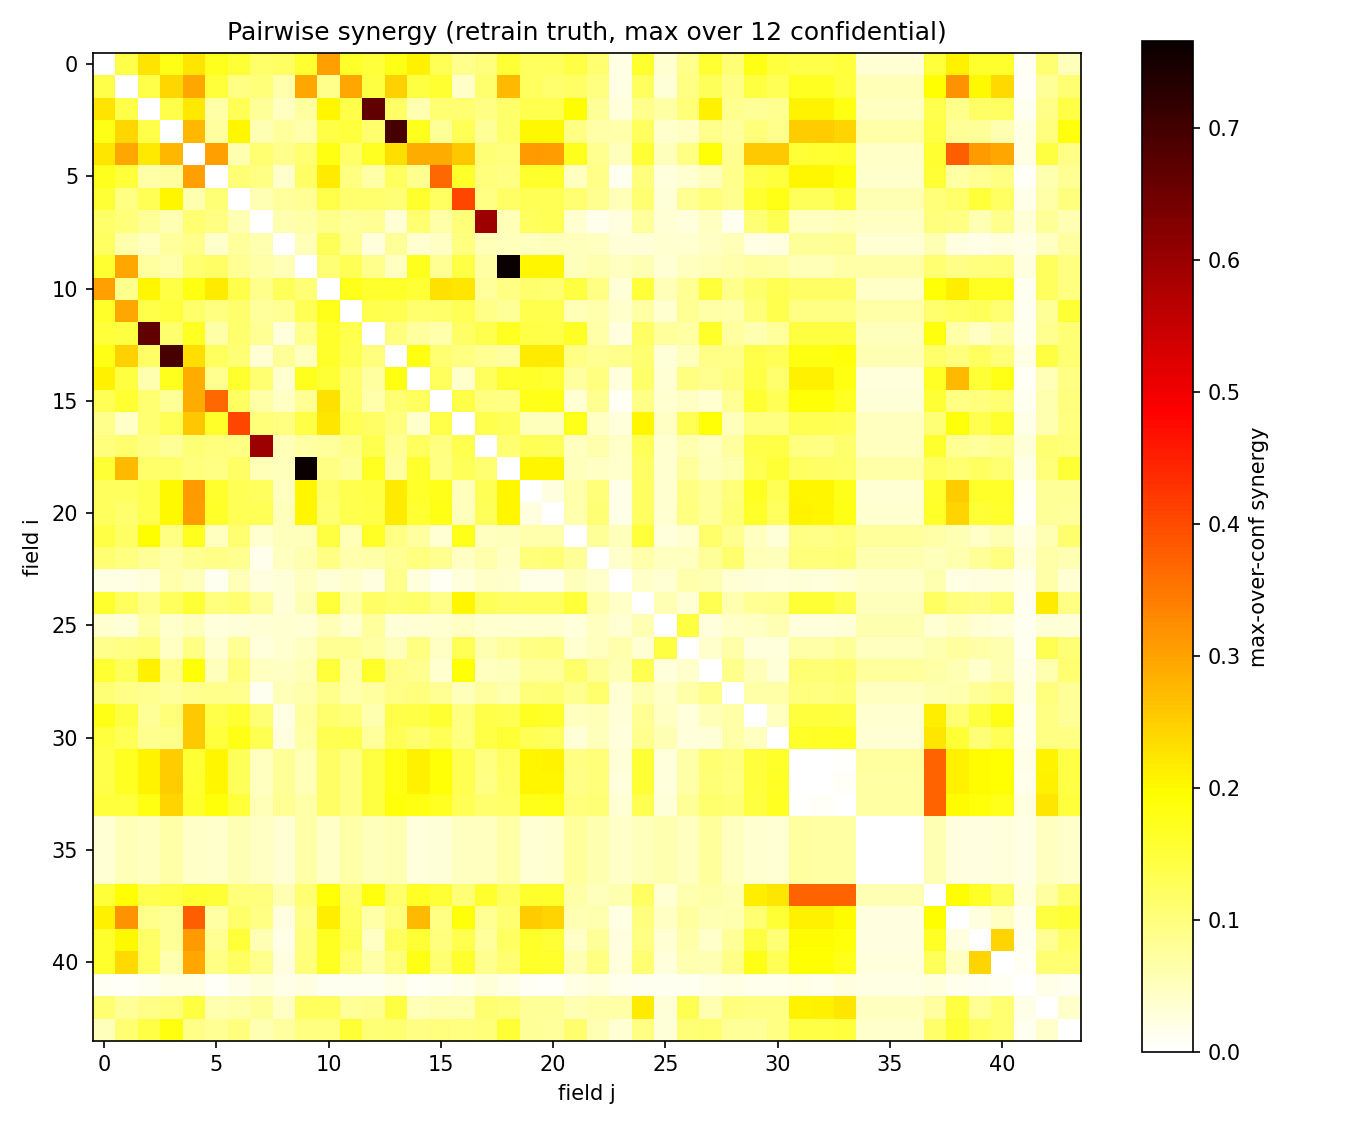
\includegraphics[width=0.70\linewidth]{synergy2_heatmap.png}}
{\heiti 图 2\quad 二阶协同图 $G_{\mathrm{syn}}$ 的邻接矩阵热力图（946 个字段对全部重训，对 12 个机密字段取最大值）。显著协同（深色）集中于少数“出力—占比”字段对，呈明显稀疏结构}
\label{fig:heatmap}
\end{figure}

\begin{table}[htbp]
\centering {\heiti 表 2\quad 最强二阶协同对（全部为重训真值）}
\vspace {1mm}
\begin{center}
\zihao{5-}
\begin{tabular}{llcccc}
\toprule
字段对 $(i,j)$ & 机密目标 $c$ & $v_c(\{i\})$ & $v_c(\{j\})$ & $v_c(\{i,j\})$ & $\mathrm{syn}_2^c$ \\
\midrule
风电出力 + 风电占比     & 总发电量 & 0.064 & 0.162 & 0.928 & \textbf{0.765} \\
多燃料出力 + 多燃料占比 & 总发电量 & 0.201 & 0.078 & 0.897 & 0.696 \\
水电出力 + 水电占比     & 总发电量 & 0.292 & 0.135 & 0.957 & 0.665 \\
太阳能出力 + 太阳能占比 & 总发电量 & 0.006 & 0.099 & 0.695 & 0.596 \\
\bottomrule
\end{tabular}
\label{tab:syn2}
\end{center}
\end{table}

\begin{observation}[单字段评分的不适定性]
表 2 中的字段在任何单字段评分体系下均属低风险（$v_c\le 0.29$），但其两两组合的泄露达 0.70--0.96。不存在仅依赖单字段分数的单调聚合规则能同时正确刻画“太阳能出力单独共享安全”与“太阳能出力与占比合体高危”两个事实——前者要求其分数低，后者要求其分数高。敏感度必须定义在集合上。
\end{observation}

\textbf{置零口径系统性失效}。在同一批字段对上按式 (\ref{eq:zero}) 计算置零协同并与重训真值对比：置零协同均值 0.012，重训真值均值 0.041，系统性低估 3.4 倍；两者排序的 Spearman 相关系数仅 0.351。即置零口径既低估绝对量、又排不对相对顺序——依赖该口径的评估会漏报几乎全部头部协同。原因正是 3.4 节的两点分析：置零样本偏离训练分布，且固定参数无法表达攻击者对可见集合的重新优化。此结果确立了本框架的测量纪律：\textbf{一切进入结论的协同数值必须来自重训认证}。

\subsection{RQ2：oracle 保真度与微调收敛}

图 3 与表 3 给出子集条件图 oracle 相对重训真值的保真度随微调步数 $K$ 的变化。三点结论：

(1) \textbf{摊销估计的排序信息在 $K=0$ 时已可用}。不微调时宽尺寸集合的排序 Spearman 相关已达 0.975，字段对为 0.962——oracle 单次前向即可胜任“哪些集合更危险”的粗排，这是扫描协议的成本下界。

(2) \textbf{微调单调闭合绝对误差}。$K$ 从 0 增至 200，宽尺寸集合逐机密字段 MAE 由 0.136 降至 0.078，字段对由 0.081 降至 0.035，三元组由 0.138 降至 0.044；三元组排序相关由 0.846 升至 0.973。三个 oracle 种子的复核结论一致，排除单一模型的偶然性。

(3) \textbf{成本压缩两个数量级}。$K=200$ 时每集合约 3.1 秒，而一次完整重训需数百轮训练（分钟级）；13244 个三元组的全扫描因此从不可行变为约 11 GPU 时。

\begin{figure}[htbp]
\centering
\centerline{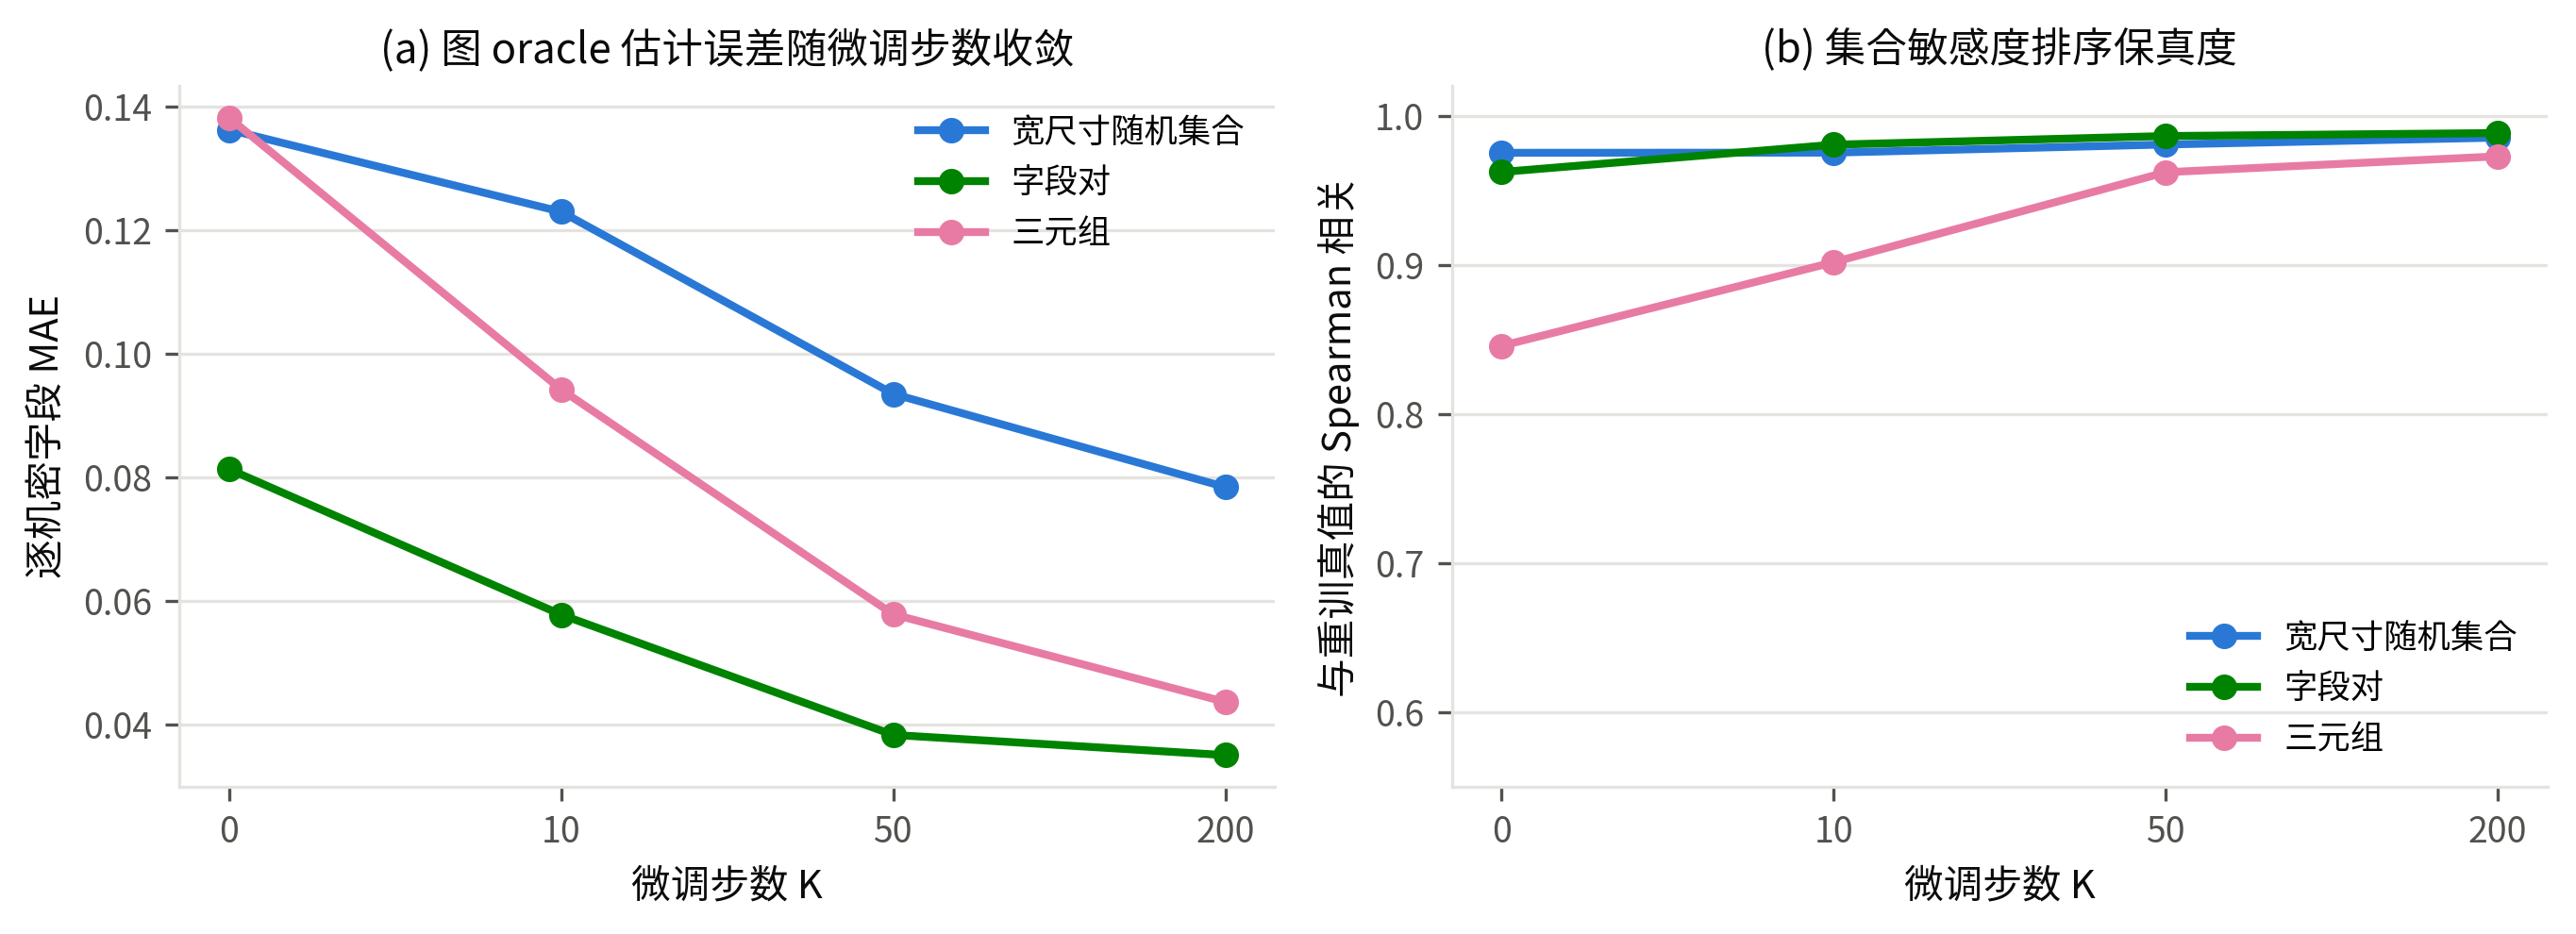
\includegraphics[width=0.98\linewidth]{oracle_fidelity_zh.png}}
{\heiti 图 3\quad 子集条件图 oracle 对重训真值的保真度随微调步数 $K$ 的收敛：(a) 逐机密字段 MAE；(b) 集合排序 Spearman 相关系数}
\label{fig:oracle}
\end{figure}

\begin{table}[htbp]
\centering {\heiti 表 3\quad 图 oracle 保真度（相对重训真值，$K$ 为微调步数）}
\vspace {1mm}
\begin{center}
\zihao{5-}
\begin{tabular}{lcccc}
\toprule
集合类别 & MAE ($K{=}0$) & MAE ($K{=}200$) & Spearman ($K{=}0$) & Spearman ($K{=}200$) \\
\midrule
宽尺寸随机集合（50 个） & 0.136 & 0.078 & 0.975 & 0.985 \\
字段对（946 个）        & 0.081 & 0.035 & 0.962 & 0.988 \\
三元组（397 个）        & 0.138 & 0.044 & 0.846 & 0.973 \\
\bottomrule
\end{tabular}
\label{tab:oracle}
\end{center}
\end{table}

\subsection{RQ3：三阶协同的全扫描与重训认证}

以 $K{=}200$ 微调 oracle 执行算法 1（$k=3$，$B_{\mathrm{top}}=200$，$B_{\mathrm{rand}}=200$，$\delta=0.10$），扫描全部 13244 个三元组并认证 397 个（top 组去重后 197 个），认证记录按（三元组，机密字段）展开共 4764 条。结果见图 4。

\begin{figure}[htbp]
\centering
\centerline{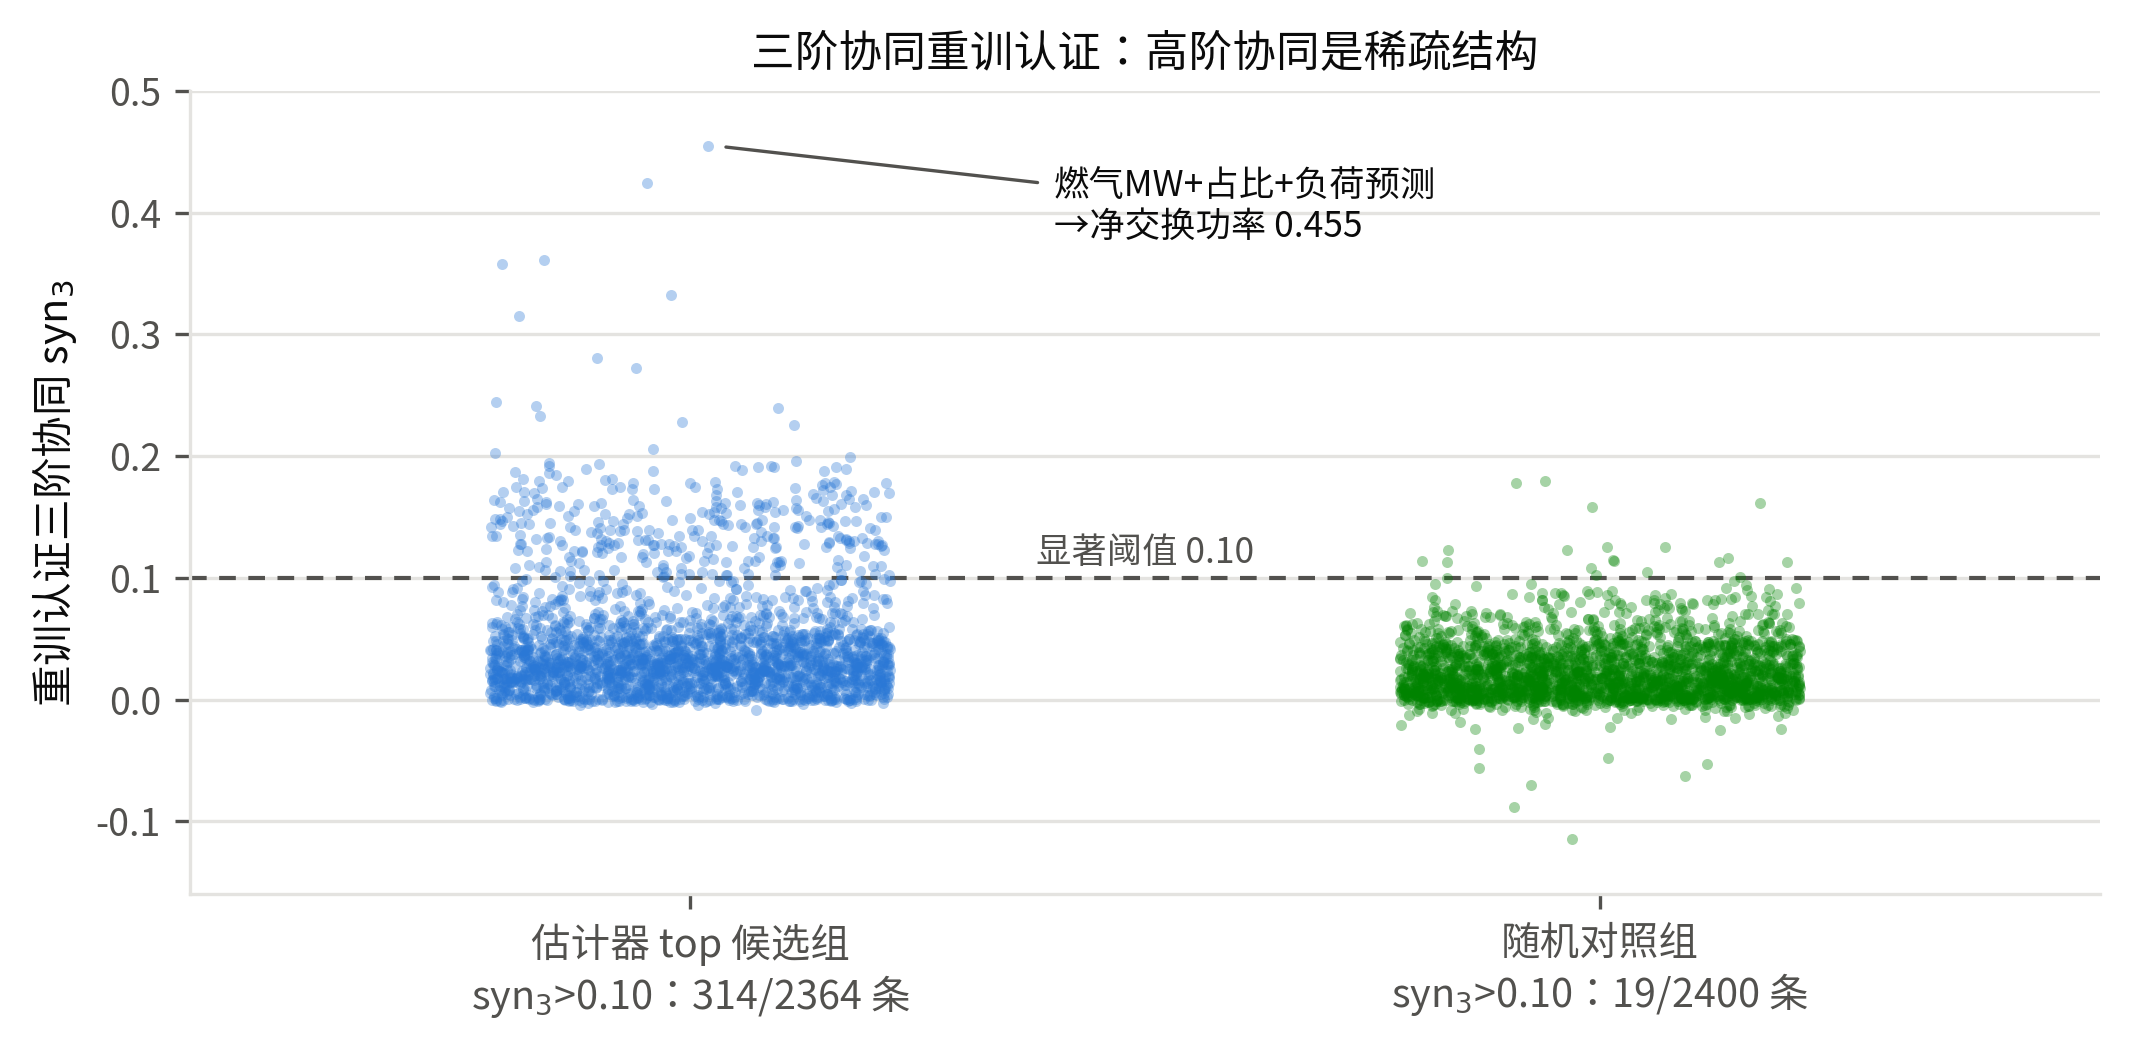
\includegraphics[width=0.85\linewidth]{triple_certify_zh.png}}
{\heiti 图 4\quad 三阶协同重训认证结果。top 候选组 2364 条认证记录中 314 条超过显著阈值 $\delta=0.10$；随机对照组 2400 条中仅 19 条，中位数 0.018 处于噪声底附近}
\label{fig:triple}
\end{figure}

\textbf{协议检验通过}。(a) 排序一致性：认证样本上估计与真值 Spearman 相关 0.795，top 筛选有效覆盖真强项；(b) 保守性成立：估计系统性不高于真值（最强项估计 0.421，认证真值 0.455），与 4.4 节的摊销残差方向分析一致，保证筛选不漏强项；(c) 稀疏性：随机对照组阳性率仅 19/2400（0.8\%），中位数 0.018 处于噪声底附近。

\textbf{真不可约三阶协同存在且物理可解释}。最强认证协同为“燃气出力 + 燃气占比 + 最新负荷预测 $\to$ 净交换功率”，$\mathrm{syn}_3=0.455$，而其三个二元子集的最优值仅 0.24--0.28。物理机制清晰：净交换功率恒等于总发电减总负荷，恢复发电需要“出力 + 占比”两字段（RQ1 的二阶机制），恢复负荷需要“负荷预测”一字段，三者缺一不可——这是超越一切二阶分析的、真正的三方合谋泄露。燃煤、核电、水电、风电的同构三元组认证值为 0.24--0.42，构成协同超图 $H_{\mathrm{syn}}$ 中结构一致的一族超边。

\textbf{稀疏性的方法学含义}。头部三阶协同集中于“低阶强协同 + 一个补全字段”的模式，而随机三元组几乎不含显著协同。这一实测稀疏性支持 4.6 节的先验式剪枝：更高阶的候选生成可以锚定在已认证的低阶超边上，使协议在阶数与字段数上均可扩展。

\subsection{RQ4：图结构的收益定位}

最后考察图结构本身带来了什么。在 50 个宽尺寸随机集合上，对每个集合分别从头重训图攻击者与多层感知机攻击者（协议完全一致），图 5 显示：图结构在 5 字段及以上的所有规模带上平均 $R^2$ 一致更高（5--8 字段带提升 0.023，超过图模型显著标尺），逐集合胜率随规模从 20\%单调升至 90\%；仅在极小集合（1--4 字段）上无优势——此时图中大量不可见节点使消息传递退化，而在 33--44 字段带两种结构同时逼近信息上限（$R^2\approx0.86$），差异自然收敛。此外两种结构存在互补性：逐机密字段取较优者可再获得 0.005--0.017 的包络增益，这正是本文以 best-of-struct 作为 $\sup$ 经验近似的依据。概言之，图结构的收益集中于中大规模集合的专用推断——集合越大，相关图先验对假设空间的约束越有效；该结论同时为攻击上限口径与后文的迁移性讨论提供了实验支点。

\begin{figure}[htbp]
\centering
\centerline{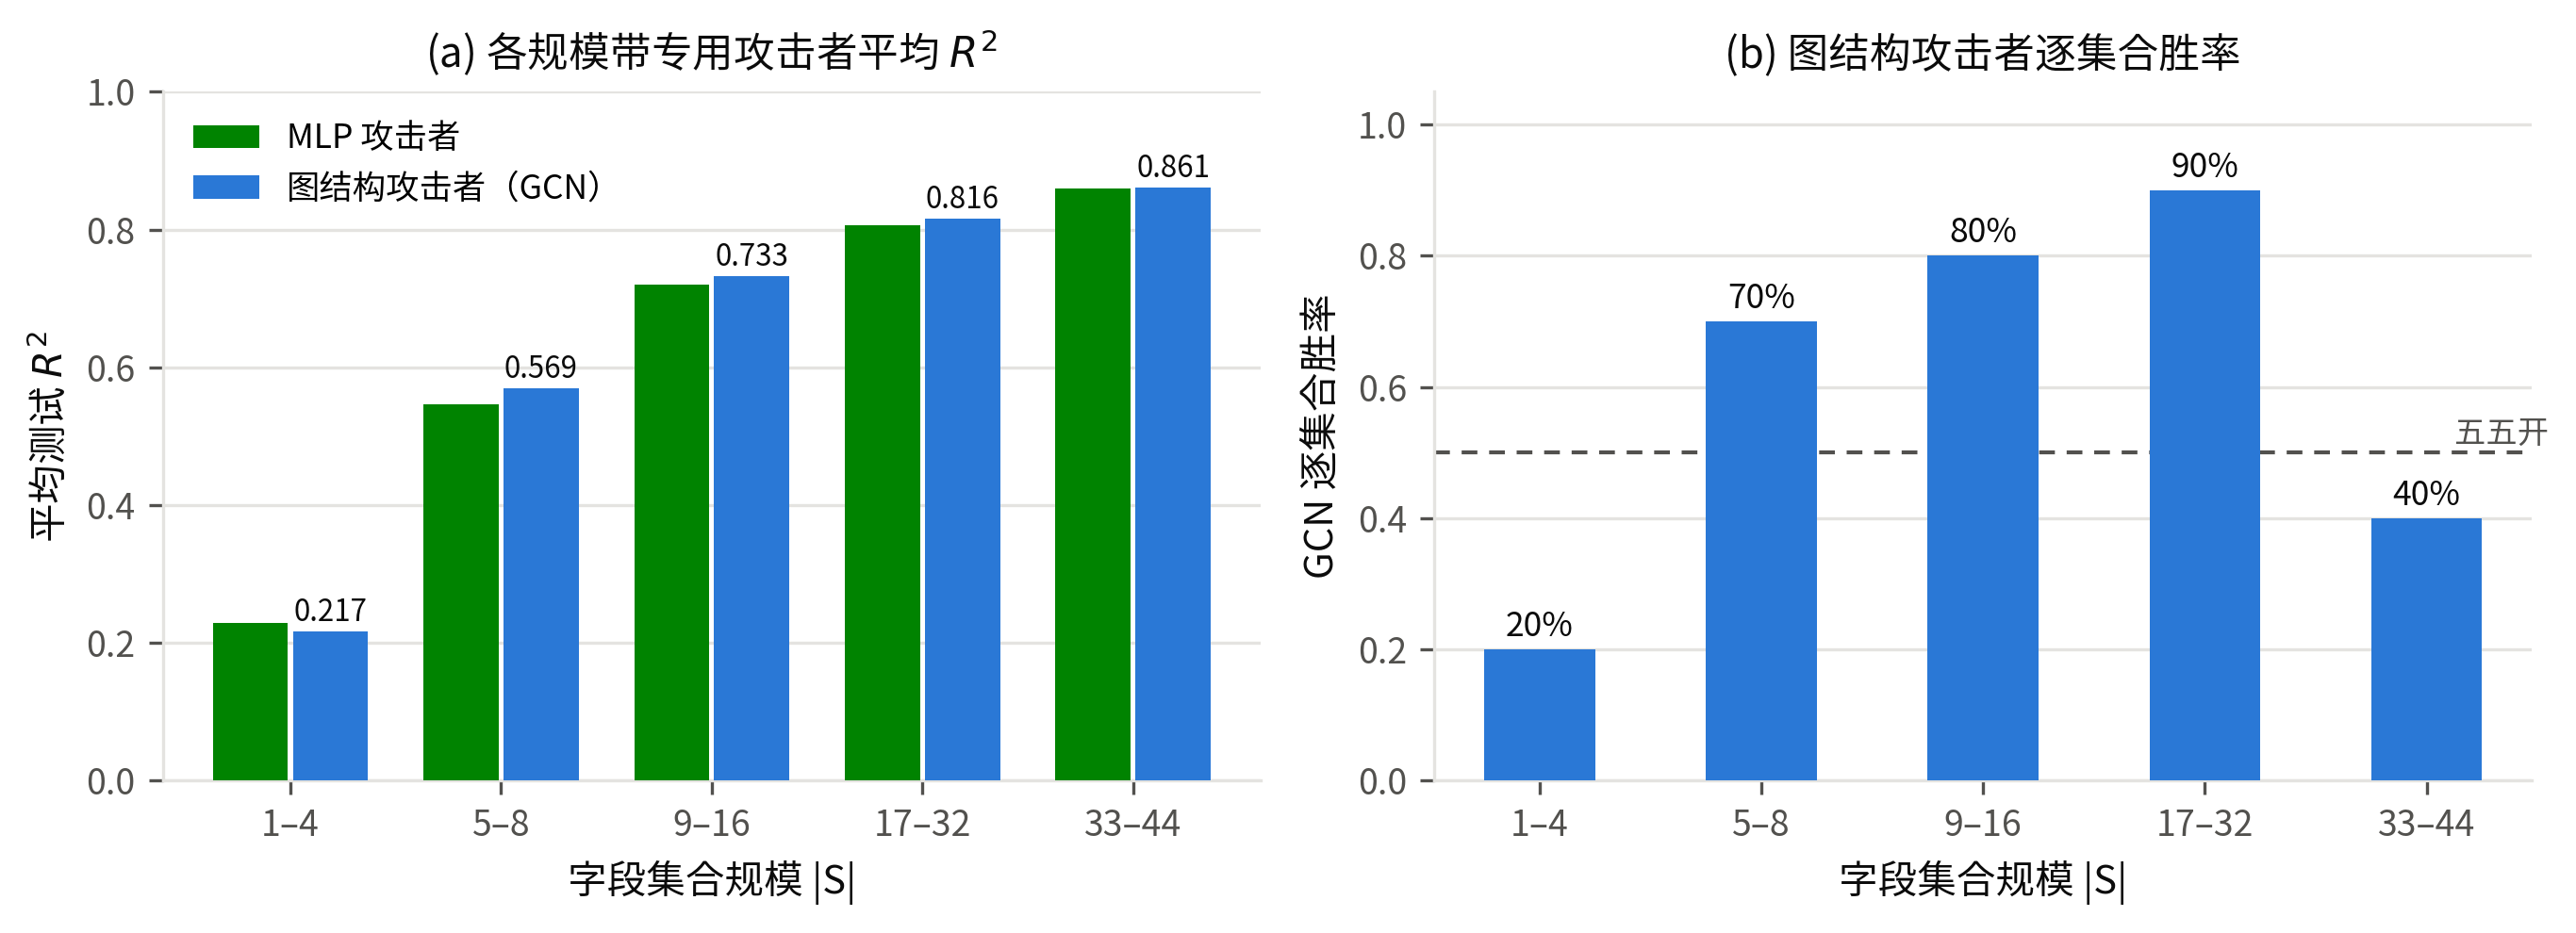
\includegraphics[width=0.98\linewidth]{attacker_compare_zh.png}}
{\heiti 图 5\quad 图结构与多层感知机专用推断模型的对比（50 个宽尺寸随机集合，逐集合重训）：(a) 各规模带平均测试 $R^2$；(b) 图模型逐集合胜率随集合规模的变化}
\label{fig:attacker}
\end{figure}

\section{\heiti 讨论}

\textbf{图结构的适用边界}。本文将图结构的收益定位在专用推断通道（RQ4），并如实指出其边界：在摊销 oracle 这一角色上，同等优化步数下无结构的多层感知机估计器在绝对误差上仍具竞争力，图 oracle 的相对优势体现为排序保真度已足够支撑扫描协议，而非逐点精度的全面领先。这与关系归纳偏置的一般规律相符\upcite{battaglia2018relational,grinsztajn2022tabular}：专用推断的依赖结构与相关图对齐，图先验获益；而“对任意掩码模式做摊销回归”更接近无结构的表格学习，结构先验的红利有限。按角色分工——图结构负责攻击上限与结构组织，摊销估计负责扫描吞吐——是本框架的务实选择。

\textbf{可迁移性}。图结构模型的参数由共享的消息函数、注意力函数与读出函数构成，与字段数量、字段顺序及字段身份解耦；节点仅需去身份化的输入（观测值与可见位）。这意味着面对字段集不同的另一电网系统，图攻击者与图 oracle 在结构上支持直接迁移或少样本适配，而多层感知机的第一层权重与字段维度一一绑定，结构上无法跨系统复用。在 IEEE 标准算例系统上开展跨系统迁移、并与 IGNN 正面对比，是本框架最自然的延伸；本文以分析性论证给出该方向，实验验证留作未来工作。

\textbf{可扩展性与低阶稀疏猜想}。RQ3 的稀疏性证据提示集合函数 $v_c(\cdot)$ 可能具有布尔函数意义上的低度数近似结构\upcite{odonnell2014boolean}：若 $v_c$ 能由单字段、显著二阶与显著三阶项良好重构，则任意集合的敏感度评估从 $2^n$ 塌缩为 $O(n^2)$--$O(n^3)$ 个已认证系数的查询与组合，且本文已备有 50 个宽尺寸随机集合真值可作为该猜想的独立检验集。结合 4.6 节的先验式剪枝，框架有望推广到字段数显著更多的系统。

\textbf{局限}。(1) 协同显著阈值 $\delta=0.10$ 是基于噪声底的经验选择，不同应用可能需要不同的风险容忍度；(2) 三阶 top 候选来自估计器扫描，尽管保守性检验通过，认证组的绝对数值仍可能带有轻微选择偏差，故稀疏性结论以随机对照组为准；(3) $\sup$ 语义以两种结构的 best-of-struct 近似，真实攻击者的模型族更大，本文数值应理解为攻击风险的\textbf{下界证词}——真实风险只会更高，这使本文的泄露警示结论更加稳健，但对“安全”的判定需保留余量。

\section{\heiti 结论}

本文针对电网数据共享中的推断泄露威胁，指出单字段敏感度评分在原理上无法刻画“单看安全、合体泄露”的协同效应，并将敏感度评估升维为任意字段集合上的集合函数 $v_c(S)$。围绕语义忠实性、组合爆炸与高阶结构定位三个挑战，本文提出以图结构为骨架的三阶段评估框架：字段相关图提供结构先验；“重训真值 + oracle 估计”双通道以两个数量级的成本压缩实现任意集合的敏感度评估（$K{=}200$ 微调后 MAE 0.078、排序 Spearman 相关 0.97 以上）；扫描—认证协议在 13244 个三元组的组合空间中定位真不可约三阶协同并给出重训证书（估计—认证排序相关 0.795 且保守）。在 PJM 真实数据上，框架产出了完整的二阶协同图与三阶协同超图：最强二阶协同“风电出力 + 风电占比 $\to$ 总发电量”达 0.765，最强三阶协同“燃气出力 + 燃气占比 + 负荷预测 $\to$ 净交换功率”达 0.455，且高阶协同被证明是稀疏、物理可解释的结构。实验同时定量否定了置零口径（低估 3.4 倍、排序相关 0.351），确立了“估计只用于筛选、结论以重训证书落地”的测量纪律。未来工作将沿两个方向推进：以低阶稀疏重构检验集合函数的可压缩性，将框架推广到更大字段规模；在标准算例系统上开展跨系统迁移，检验图结构参数与字段身份解耦所带来的可迁移性。

%%%%%%%%%%%%%%%%%%%%%%%%%%%%%%%%%
\vspace {10mm}
\centerline
{\zihao{5}\textsf{参~考~文~献}}
\zihao{5-} \addtolength{\itemsep}{-1em}
\vspace {1.5mm}
\bibliographystyle{gbt7714-numerical}
\bibliography{ref.bib}

\end{document}
